%%%%%%%%%%%%%%%%%%%%%%%%%%%%%%%%%%%%%%%%%%%%%%%%%%%%%%%%%%%%%%%%%%%%%%
% Dual Trace Communication Event Analysis
% 
% Author: Nora Huang
% Date: July 2017
% 
%%%%%%%%%%%%%%%%%%%%%%%%%%%%%%%%%%%%%%%%%%%%%%%%%%%%%%%%%%%%%%%%%%%%%%

\documentclass[paper=a4, fontsize=11pt]{scrartcl}
\usepackage[T1]{fontenc}
\usepackage{fourier}
\usepackage{tabu}
\usepackage{float}
\usepackage{afterpage}
\usepackage{booktabs}

\usepackage{longtable}
\usepackage{multicol}
\usepackage{multirow}

\usepackage[english]{babel}															% English language/hyphenation
\usepackage[protrusion=true,expansion=true]{microtype}	
\usepackage{amsmath,amsfonts,amsthm} % Math packages
\usepackage[pdftex]{graphicx}	
\usepackage{url}
\usepackage{listings}
\lstset{
    frame=single,
    breaklines=true
}


%%% Custom sectioning
\usepackage{sectsty}
\allsectionsfont{\centering \normalfont\scshape}


%%% Custom headers/footers (fancyhdr package)
\usepackage{fancyhdr}
\pagestyle{fancyplain}
\fancyhead{}											% No page header
\fancyfoot[L]{}											% Empty 
\fancyfoot[C]{}											% Empty
\fancyfoot[R]{\thepage}									% Pagenumbering
\renewcommand{\headrulewidth}{0pt}			% Remove header underlines
\renewcommand{\footrulewidth}{0pt}				% Remove footer underlines
\setlength{\headheight}{13.6pt}


%%% Equation and float numbering
\numberwithin{equation}{section}		% Equationnumbering: section.eq#
\numberwithin{figure}{section}			% Figurenumbering: section.fig#
\numberwithin{table}{section}				% Tablenumbering: section.tab#


%%% Maketitle metadata
\newcommand{\horrule}[1]{\rule{\linewidth}{#1}} 	% Horizontal rule

\title{
		%\vspace{-1in} 	
		\usefont{OT1}{bch}{b}{n}
		\normalfont \normalsize \textsc{Department of Computer Science,  University of Victoria} \\ [25pt]
		\horrule{0.5pt} \\[0.4cm]
		\huge Dual Trace Communication Event Analysis  \\
		\horrule{2pt} \\[0.5cm]
}
\author{
		\normalfont 								\normalsize
        Nora Huang\\[-3pt]		\normalsize
        \today
}
\date{}


%%% Begin document
\begin{document}
\maketitle

\section{Introduction}
Many network application vulnerabilities occur not just in one application, but in how they interact with other systems. These kinds of vulnerabilities can be difficult to analyze. Dual-trace analysis is one approach that helps the security engineers to detect the vulnerabilities in the interactive software. A dual-trace consist of two execution traces that are generated from two interacting applications. Each of these traces contains information including CPU instructions, register and memory changes of the running application. Communication information of the interacting applications is captured as the register or memory changes on their respective sides. Our research focuses on building a model to visualize and analyze dual-trace which would be available for various kinds of communication type.

\section{Problem}
The major problem we are considering in dual-trace analysis is locating the communication events in the traces from both sides and present them to the user. In order to do so,  we first, have to develop a method to locate those events in the traces, and second, develop an user interface for accessing the communication event information.\par

Before jumping into solving the problem we need to define what is a communication event. In this work, a communication event in the dual trace is defined as a successfully send and received message. There are four essential elements in this event: send function call, receive function call, the sent message in the sender's memory and the received message in the receiver's memory. However, in some cases, the send and receive operation are not always exactly paired. For example, the receiver buffer is small than the sender buffer, the receive function has to be called multiple times to receive one message from the sender. In this case, the one send to multiple receive event is broken into multiple send and receive events as shown in Figure \ref{event}. 

\begin{figure}[h]
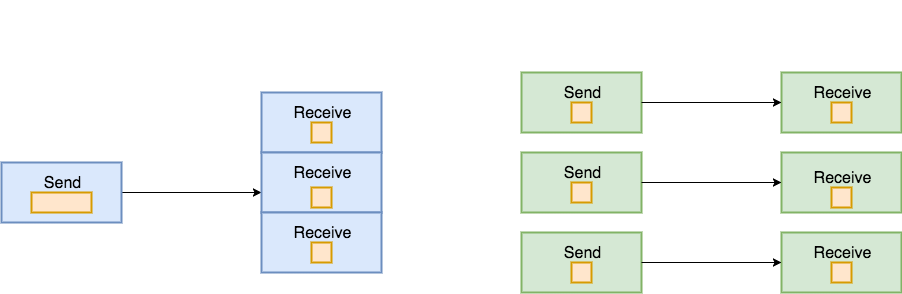
\includegraphics[scale=.415]{event}
 \caption{Break one send/multiple receive into multiple send/receive events}
\label{event}
\end{figure}

\section{Communication Types}
In order to synchronize the messaging of both side of the traces, we need to investigate the communication methods to figure out how they looks like in the assembly level traces.
There are so many communication methods exists in the real world. We are not covering all of them at a time, but start from narrowing down our study into some sort of communication methods. Transport channels in windows communication framework including named pipes, MSMQ, HTTP and TCP channels are targeted in this work in the first phase. And it is possible to extend it for more general use cases.
\subsection{Assembly Calling Convention}
Before we jumping into a specific communication method, it is important to know some basic assembly calling convention.
Calling Convention is different for operating system and the programming language. Since we are looking into the messaging methods being used in windows communication framework, and since our case study is running on a Microsoft* x64 system, we only list the Microsoft* x64 calling convention for interfacing with C/C++ style functions:\par
\begin{enumerate}  
\item RCX, RDX, R8, R9 are used for integer and pointer arguments in that order left to right.
\item XMM0, 1, 2, and 3 are used for floating point arguments.
\item Additional arguments are pushed on the stack left to right. \ldots 
\item Parameters less than 64 bits long are not zero extended; the high bits contain garbage.
\item Integer return values (similar to x86) are returned in RAX if 64 bits or less.
\item Floating point return values are returned in XMM0.
\item Larger return values (structs) have space allocated on the stack by the caller, and RCX then contains a pointer to the return space when the callee is called. Register usage for integer parameters is then pushed one to the right. RAX returns this address to the caller.
\end{enumerate}

\subsection{Named pipes Channel}
A named pipe is a named, one-way or duplex pipe for communication between the pipe server and one or more pipe clients. All instances of the named pipe share the same pipe name, but each instance has its own buffers and handlers. In here we only consider one to one server/client pairs. One server to multiple clients scenario can always be broken into multiple server/client pairs. To locate a named pipe message event in dual-trace, we need to know how the channels are created as well as how the messages are send and received in the assembly traces. The creation of a named pipe will return the handler of that pipe. This handler will be used later on when messages are being sent or received. So we need to know the function calls for named pipe creation and message send/receive to locate the event in the traces. In the follow subsections, we will list the related functions for the named pipe channel for both synchronous mode and asynchronous mode. The create channel functions for both modes are the same but with different input parameters. The functions for send and receive message are also the same for both case. However, the operation of the send and receive functions are different for different mode. In addition, extra function are being called to check the status of message sending or receiving in asynchronous mode as well as the message content.
\subsubsection{Synchronous}
We list all the functions that needed to locate an messaging event in a dual-trace in Table\ref{synfunctions} for synchronous named pipe. The Channel Create Functions indicate how the channel being created in server and client sides, and the mattered parameters. For named pipes the channel create functions are different between in server and client. The parameter in RDX can indicate if the channel is opened as synchronous mode. The send or receive message functions are the same in server and client. When the channel is being created, the input file names for a channel at server and the client are the same, but the returned File Handler IDs are different. The send and receive function only use the handler to send and receive message to a specific channel. 
\begin{table}[h]
        \centering
        \caption{Functions for communication type definition of synchronous named pipe}
        \label{synfunctions}
        \begin{tabular}{|l|l|l|l|l|l|l|}
            \hline
             \multirow{2}{*}{} &
               \multicolumn{2}{c|}{Channel Create Functions} &
               \multicolumn{2}{c|}{Message Send Functions} &
               \multicolumn{2}{c|}{Message Receive Functions} \\
             \cline{2-7}
              & Function& Parameters & Function & Parameters  & Function & Parameters\\
             \hline
             Sever& Create-&  RAX: File Handler &  &  RCX: File Handler &&RCX: File Handler\\
             \cline{3-3} \cline{5-5} \cline{7-7}
             &NamedPipe&RCX: File Name && RDX:  &&RDX: \\
              \cline{3-3} 
             &&RDX: Asyn/Syn&WriteFile & Buffer Address &ReadFile&Buffer Address\\
                \cline{1-3} \cline{5-5} \cline{7-7}
             Client & CreateFile & RAX: File Handler & &  R8: Buffer Length &&R8: Buffer Length\\
              \cline{3-3} \cline{5-5} \cline{7-7}
             &&RCX: File Name &&Stack:&&Stack:\\
             \cline{3-3} 
             &&RDX: Asyn/Syn&& Overlap Pointer&&Overlap Pointer\\
            \hline
        \end{tabular}
    \end{table}
\subsubsection{Asynchronous}
The functions used in Asynchronous mode for create channel, send and receive message are the same as those used in synchronous mode. However,  the ReadFile and WriteFile functions run asynchronously when the channel is asynchronous. This means the function will return immediately, even if the operation has not been completed. If the operation is complete when the function returns, the return value indicates the success or failure of the operation. Otherwise the functions return zero and GetLastError returns ERROR\_IO\_PENDING. In this case, the calling thread must wait until the operation has finished. The calling thread must then call the GetOverlappedResult function to determine the results. This means besides looking for ReadFile and WriteFile function calls in the traces, the GetOverlappedResult function should be checked in the traces to get the full result of the ReadFile or WriteFile operations. Table\ref{asynfunctions} list the interested parameters of the GetOverlappedResult funciton. However, it's complicated to define the communication types with so many functions for only an event. In order to make the user interface clear and simple. We ask the user to make separate definition for the follow function with the send function as a new communication type. Table \ref{Additionalfunction} shows the addition communication type for asynchronous mode.

\begin{table}[h]
        \centering
        \caption{Functions for addition communication type definition of asynchronous named pipe}
        \label{synfunctions}
        \begin{tabular}{|l|l|l|l|l|l|l|}
            \hline
             \multirow{2}{*}{} &
               \multicolumn{2}{c|}{Channel Create Functions} &
               \multicolumn{2}{c|}{Message Send Functions} &
               \multicolumn{2}{c|}{Message Receive Functions} \\
             \cline{2-7}
              & Function& Parameters & Function & Parameters  & Function & Parameters\\
             \hline
             Sever& Create-&  RAX: File Handler &  &  RCX: File Handler &&RCX: \\
             \cline{3-3} \cline{5-5} 
             &NamedPipe&RCX: File Name && RDX:  && File Handler\\
              \cline{3-3} 
             &&RDX: Asyn/Syn&WriteFile& Buffer Address &GetOverlapped-&\\
                \cline{1-3} \cline{5-5} \cline{7-7}
             Client & CreateFile & RAX: File Handler & &  R8: Buffer Length &Result&RDX:\\
              \cline{3-3} \cline{5-5} 
             &&RCX: File Name &&Stack:&&Overlap\\
             \cline{3-3} 
             &&RDX: Asyn/Syn&& Overlap Pointer&&structure\\
            \hline
        \end{tabular}
    \end{table}
    

\subsection{MQMS Channel}
\subsubsection{Synchronous}
\subsubsection{Asynchronous}

\subsection{TCP/UDP Channel}
\subsection{HTTP Channel}

\section{Prototype Building}
In this section we discuss the design of the prototype of dual-trace analysis. This prototype consist of three main components: user interface for defining the communication type, algorithm of locating the communication events in the dual-trace, user interface and strategy to navigate the located events to the sender and receiver traces. We provide the background information of the design of each component as well as their detail design in each corresponding subsection.
\subsection{User Defined Communication Type}
In our design, we don't specify any predefined communication type but give the user ability to do that. By the user interface implemented, the user can defined their own communication type. This give the flexibility to the user to define what they are looking for. Each communication type consist of 4 system function calls. They are channel create/open in sender and receiver sides, sender's send message function and receiver's receive message function. By indicating the channel create/open functions in both sender and receiver sides, the tool can acquire the channel's identifiers. Later on the tool can match the send and received messages within a specific channel. The send and receive functions are used to located the event happened in the traces. The messages sent and received are reconstructed from the memory state when the send and receive functions are called and returned. The detail of the match algorithm will be discuss later.

\subsubsection{Function Calls in the Traces}
The called functions' name can be inspected  by  search of the symbolic name in the executable binary or any DLLs which used by the program at the time when it is traced. This functionality exists in the current Atlantis. By importing the DLLs and execution  executable binary, Atlantis can list all called functions for the users in the Functions view. From this list, users can chose the interested functions and generate their interested communication type. In Figure\ref{functionsview} there is  an action item "Add to Communication type" in the right click menu of the function entry. Figure \ref{dialog} shows the dialogue for entering the information for the adding function. As this figure shows, users can get the existing communication type list in the drop down menu. They can choose to add the current function to an exist communication type or they can add it to a new communication type by entering a new name. For the channel create/open function, the register holding the address of channel's name as input and the register holding the handle identification of the channel as output are required. For the send/receive function, the register holding the address of the send/receiver buffer, the register holding the length of the sending/receiving message and the register holding the channel's identification are required. As there are 4 functions for each communication type users have to repeat this add function to communication type action for 4 times to generate one communication type.

\begin{figure}[h]
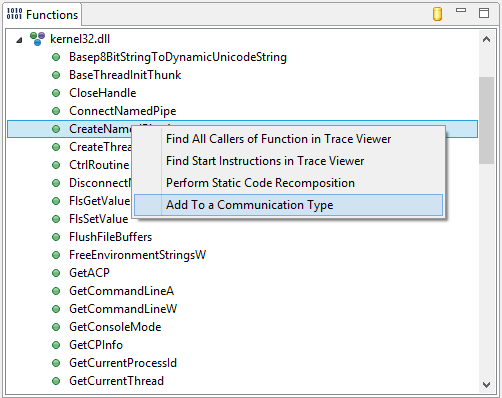
\includegraphics{functionsview}
 \caption{Add function to a Communication type from Functions View}
\label{functionsview}
\end{figure}

\begin{figure}[h]
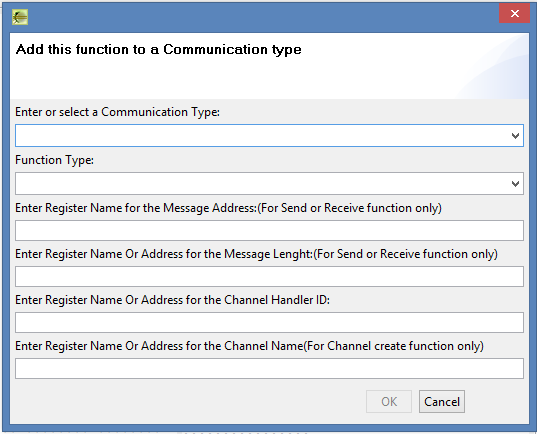
\includegraphics{dialog}
 \caption{Dialog to input information for a function adding to a communication type}
\label{dialog}
\end{figure}

\subsubsection{Communication Type Data Structure}
The defined communication type will be stored in a xml file. The list below shows the data structure of one communication type. 
\begin{lstlisting}
<messageTypesData>
    <parentFolder>.tmp</parentFolder>
    <messageTypes>
        <messageType>
            <name>namedPipe_clientsend</name>
            <sendFunction>
                <associatedFileName>Client</associatedFileName>
                <name>WriteFile</name>
                <messageAddress>RDX</messageAddress>
                <messageLengthAddress>R8</messageLengthAddress>
                <channelIdReg>RCX</channelIdReg>
            </sendFunction>
            <receiveFunction>
                <associatedFileName>Server</associatedFileName>
                <name>ReadFile</name>
                <messageAddress>RDX</messageAddress>
                <messageLengthAddress>R8</messageLengthAddress>
                <channelIdReg>RCX</channelIdReg>
            </receiveFunction>
            <sendChannelCreateFunction>
                <associatedFileName>Client</associatedFileName>
                <name>CreateFileA</name>
                <channelIdReg>RAX</channelIdReg>
                <channelNameAddress>RCX</channelNameAddress>
            </sendChannelCreateFunction>
            <receiveChannelCreateFunction>
                <associatedFileName>Server</associatedFileName>
                <name>CreateNamedPipeA</name>
                <channelIdReg>RAX</channelIdReg>
                <channelNameAddress>RCX</channelNameAddress>
            </receiveChannelCreateFunction>
        </messageType>
    </messageTypes>
</messageTypesData>
\end{lstlisting}


\subsubsection{Communication Type View}
A new view named Communication Types view is for the user defined communication types. All user defined communication type are stored in the .xml file and listed in communication type view when it's opened as shown in Figure \ref{CommunicationTypeview}. User can change the name of a communication type, remove an existing communication type or searching of the match message occurrences of selected communication type by selecting action item in the right click menu of an communication type entry. The matched messages are listed in the result window of the view. By clicking the entry of the search  result, user can navigate to it's sender or receiver's corresponding instruction line as shown in Figure\ref{searchresult}. Message content in the memory view will be shown as well.


\begin{figure}[h]
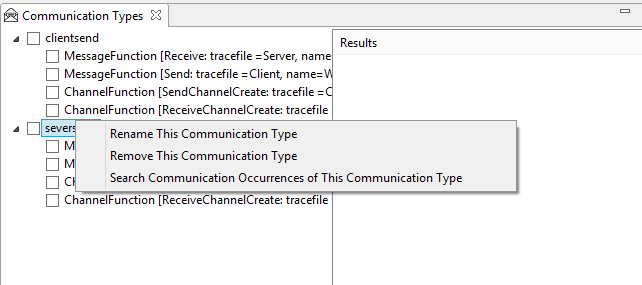
\includegraphics[scale=.9]{CommunicationTypeview}
 \caption{New View: Communication Type View}
\label{CommunicationTypeview}
\end{figure}

\begin{figure}[h]
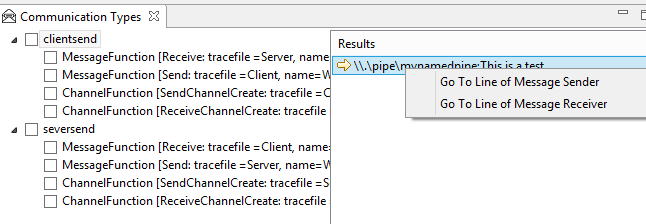
\includegraphics[scale=.9]{searchresult}
 \caption{Right Click menu to navigate to send and receive event in the traces}
\label{searchresult}
\end{figure}

\subsection{Communication Event Searching}
The communication event consists of the send message event in the sender side and receive message event in the receiver side. The communication event searching algorithm can be divided into three main steps: 1. search all channel create/open event in the sender and receiver side, save the handle id and corresponding channel name. 2. Search all message send and receive event in sender and receiver sides. 3. Matching the send/receive messages pair based on the channel names and message contents.
\subsubsection{Record opened Channel}
In this step the algorithm is supposed to search all the open channel both in the sender and receiver side. The found created channels are recorded in a map. The key of the map is the handler id of the channel and the value is the channel name. A channel in the sender and receiver sides will have different handler id but same channel name.
\subsubsection{Search send and receive Message}
All send message and receive message function calls will be found out in the trace. When a send function hit, the memory state of the hit instruction line will be reconstructed, and the message content can be get from the memory with the send message buffer address. When a receive function hit, the return line of that function is needed for getting the message content. The memory state of the function return line is reconstructed and the message content can be get  from the reconstructed memory state with the receive message buffer address.
\subsubsection{Matching the send/receive messages pair}
After the created channel and send/receive message are found out in the sender and receiver side, a matching algorithm is used to match the send/receive message pairs.
\subsubsection{Matching Event Data Structure}
The matching event is stored in cache when the tool is running. Only the most recent search result is cached currently. If users need the previous result, they need to apply the search again. The matching Event consist of two sub-events, one is message send event while the other is message receive event. Both of these two sub-events are object of BfvFileMessageMatch. BfvFileMessageMatch is an Java class extends org.eclipse.search.internal.ui.text.FileMatch. FileMatch class containing the information needed to navigate to the trace file editor. In order to show the corresponding send/receive message in the memory view, the target memory address storing the message content is set in BfvFileMessageMatch. Two more elements: message and channel name are also set in BfvFileMessageMatch which are listed in the search result. 

\subsection{Matching Event Visualization and Navigation}
The right click menu of an entry in the search result list has two action items: Go To Line of Message Sender and Go To Line of Message Receiver. Both of the action items allow users to navigate to the trace Instruction view. When the user click on these items, it will navigate to the corresponding trace sender or receiver trace instruction view.  Meanwhile the memory view jumps to the target address of the message buffer, and the memory state is reconstructed so that the message content in that buffer will be shown in the memory view.


\section{Case Study}
The case we used to test this prototype contains one named pipe synchronous channel between a server and a client. Client send a message to the server and server reply another message to the client. 
\subsection{Test and Verification Design}
The test cases are designed to find all the messages from client to server and all the messages from server to client. Two end to end test cases are designed for both scenarios. 

In each test case, there are three test steps: 1. define the communication type by adding channel creating functions and message send/receive functions of server and client sides. 2. search for the events of  the defined communication type. 3. for the occurrence of the events, navigate to the trace instruction and memory view.

Verification points are specified for each step as: 1. verify the communication types with their functions are listed in the communication view. 2. verify the message events in the dual-trace can be found and listed in the search result view. 3. verify the navigation from the result entry to the instruction view of sender trace and receiver trace.
\subsection{Result}
We used the dual-trace provided by DRDC and follow the experiment and verification design to conduct this test. Figure\ref{addcomtyperesult} shows that the user defined clientsend and serversend communication types are shown in the communication type view as well as the functions consist of the communication types. Figure\ref{occclientresult} shows the search result of clientsend communication type, while Figure\ref{occclientresult} shows the search result of the serversend communication type. By clicking the Go To Line of Message Sender and Go To Line of Message Receiver action items, instruction view and memory view updated correctly. Figure\ref{send} shows the server was sending out a message: This is an answer. 


\begin{figure}[H]
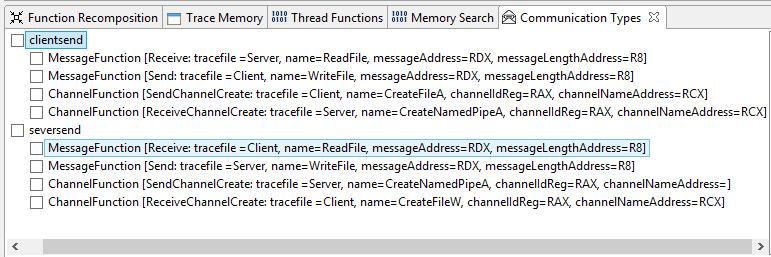
\includegraphics[scale=.72]{addcomtyperesult}
 \caption{Defined clientsend and serversend communication types in Communication View}
\label{addcomtyperesult}
\end{figure}

\begin{figure}[H]
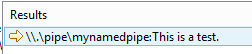
\includegraphics{occclientresult}
 \caption{the search result of clientsend communication type}
\label{occclientresult}
\end{figure}


\begin{figure}[H]
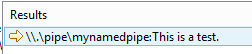
\includegraphics{occclientresult}
 \caption{the search result of the serversend communication type}
\label{occclientresult}
\end{figure}

\begin{figure}[H]
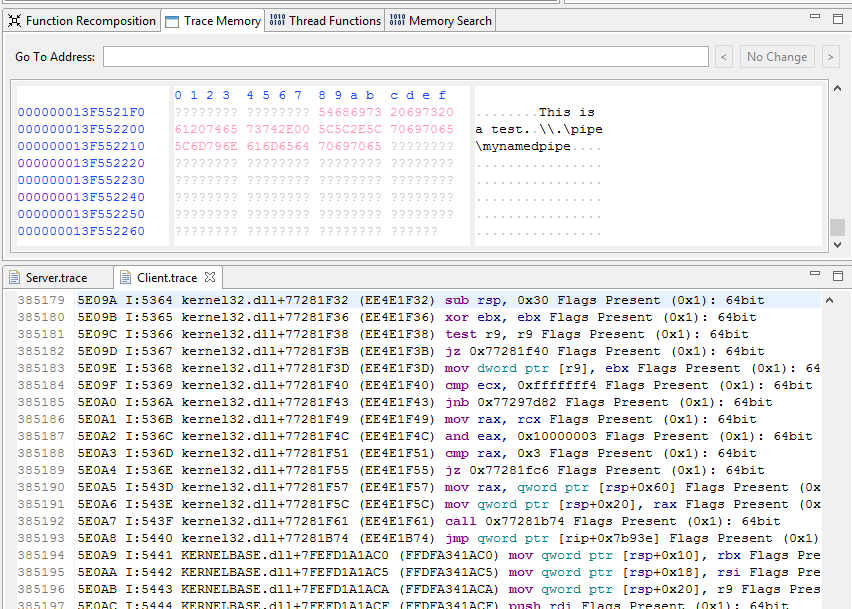
\includegraphics[scale=.66]{send}
 \caption{instruction view and memory view updated correctly}
\label{send}
\end{figure}

\subsection{Time Analysis}
\subsection{Conclusion}
\section{Limitations}
In this section, we specify the limitations of the current prototype and the reasons for them. 
\subsection{Event Status: Success or Fail}
In current prototype, we only consider the success cases. For the Fail case, since the message was not successfully sent or received, there are high chance that they are not existed in the memory of the trace. From the assembly level trace, if the message was not traced in the memory, there is no way to match the sent/received message pair in the trace analysis.   

\subsection{Match Events Distinguishing}
Distinguishing is considered when multiple clients connecting to the same server. Each connection is considered as an instance. In the server side all this instances have the same pipe name but different handler ID. However in the assembly trace level there is no way to match a client with it instance handler ID. In consequence, if the same content messages are being sent/received by different clients, when the user want to match the message pair between a client and the server, there is no way to distinguish the correct one from the assembly trace level. As a result, our tool will list all the matched content message event, regardless if it's from the interested client. The user can distinguish the correct ones for this client, if they have extra information.

\subsection{Match Events Ordering}
Ordering is considered when multiple messages with exactly the same content being send/receive between the client and server. If the channel is synchronous, the order of the event is always consist with the order they happen in both the sender and receive sides. However for the asynchronous channel, there are chance that the sent messages in the sender side's trace are out of order with the received messages in the received side's trace. Unfortunately, There is no way in the assembly level trace to match the exactly ones. As a result, our tool can only order the event based on the order they happen in the traces.

\subsection{Buffer Sizes Of Sender and Receiver Mismatch}
In current prototype, we only consider the success cases. For the Fail case, since the message was not successfully sent or received, there are high chance that they are not existed in the memory of the trace. From the assembly level trace, if the message was not traced in the memory, there is no way to match the sent/received message pair in the trace analysis. 

\section{Future Work}


\bibliographystyle{abbrv}
\bibliography{referencelist} 


%%% End document
\end{document}